\documentclass[addpoints]{exam}

\usepackage[utf8]{inputenc}
\usepackage{float}
\usepackage{geometry}
\usepackage{amssymb}
\usepackage{amsthm}
\usepackage{amsmath}
\usepackage{graphicx}
\usepackage[breaklinks]{hyperref}
\usepackage{listings}
\usepackage{fancyhdr}
\usepackage[english]{babel}
\usepackage{mdframed}
\usepackage{bookmark}
\usepackage{lipsum}
\usepackage{color, xcolor, colortbl, longtable}
\usepackage{psfrag}
\usepackage{pgfplots}
\usepackage{titlesec}
\usepackage{cite}
\usepackage{hyperref}
\usepackage{tabularx}
\usepackage{pythonhighlight, pifont}
\usepackage{pagerange}
\usepackage{venndiagram}
\usepackage{multicol}
\usepackage{multirow}
\usepackage{array}
\usepackage{url}
\usepackage{pagerange}
\usepackage[shortlabels]{enumitem}
\newtheorem{theorem}{Theorem}

% Defining a light gray color for row headers

\definecolor{light-gray}{gray}{0.75}

% Header and footer.
\pagestyle{headandfoot}
\runningheadrule
\runningfootrule
\runningheader{MGMT 323}{Supply Chain Managment}{Assignment 01}
% \runningfooter{}{Page \thepage\ of }{}
\runningfooter{}{\thepage \;of 7}{}
\firstpageheader{}{}{}

\boxedpoints
\printanswers
% \qformat{} %Comment this to number questions, uncomment this to not number questions

\newcommand\union\cup
\newcommand\inter\cap
\newcommand{\N}{\mathbb{N}}
\newcommand{\Z}{\mathbb{Z}}
\newcommand{\olsi}[1]{\,\overline{\!{#1}}} % overline short italic

\title{MGMT 323 - Supply Chain Management}
\author{Assignment 01}
\date{Ali Muhammad Asad - aa07190}

\pgfplotsset{compat=1.18}

\begin{document}
\maketitle
\begin{sloppypar}
\section*{Make or Buy Decision}
\begin{questions}
    \question Your are given the following information:
    \begin{figure}[ht]
        \centering
        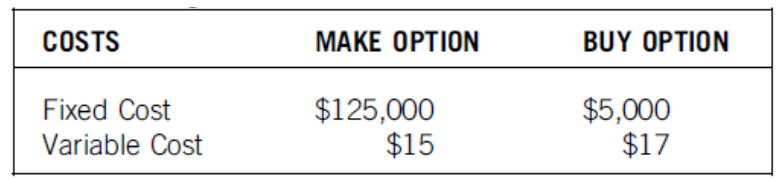
\includegraphics[width=0.5\textwidth]{q1.png}
    \end{figure}
    \begin{enumerate}
        \item[a.] Find the break-even quantity and the total cost at the break-even point.
        \item[b.] If the requirement is 150,000 units, is it more cost-effective for the firm to buy or make the components? What is the cost savings for choosing the cheaper option?
    \end{enumerate}
    \begin{solution}
        \begin{enumerate}
            \item[a.] $ Q_{BE} = \displaystyle\frac{F_M - F_B}{V_B - V_M} = \displaystyle\frac{125000 - 5000}{17 - 15} = \displaystyle\frac{120000}{2} = 60000 $
            
            The breakeven quantity is 60,000 units.
            
            Total Cost = $ 125000 + 15(60000) = \$1025000 $

            \item[b.] For a requirement of 150000 units, the breakeven quantity is less than the requirement. Therefore, it is more cost-effective for the firm to make the components.
            
            Cost if firm makes the components = $ 125000 + 15(150000) = \$2375000 $

            Cost if firm buys the components = $ 5000 + 17(150000) = \$2555000 $

            Cost savings = $ 2555000 - 2375000 = \$180000 $

            The firm saves \$180,000 by making the components.
        \end{enumerate}
    \end{solution}

    \pagebreak
    \question Ms. Jane Kim, Purchasing Manager of Kuantan ATV, Inc., is negotiating a contract to buy 20,000 units of a common component part from a supplier. Ms. Kim has done a preliminary cost analysis on manufacturing the part in-house and concluded that she would need to invest \$50,000 in capital equipment and incur a variable cost of \$25 per unit to manufacture the part in-house. Assuming the total fixed cost to draft a contract with her supplier is \$1,000, what is the maximum purchase price that she should negotiate with her supplier? What other factors should she negotiate with the suppliers?
    \begin{solution}
        For the given scenario, we can construct the following table:
        \begin{center}
            \begin{tabular}{|c|c|c|}
                \hline \textbf{Costs} & \textbf{Make Option} & \textbf{Buy Option} \\ \hline
                Fixed & 50000 & 1000 \\ \hline
                Variable & 25 & x \\ \hline
            \end{tabular}
        \end{center}
        Now we have 20,000 units. 

        Cost for Make = $ 50000 + 25(20000) = 50000 + 500000 = 550000 $

        Cost for Buy = $ 1000 + 20000x $

        Then we can find the maximum purchase price for her to negotiate as so: \\ 
        $ 1000 + 20000x < 550000 \implies x < 27.45 $. 

        Then the maximum purchase price she should negotiate with her supplier is \$27.45 as after \$27.45, it would be more cost-effective for her to make the components in-house as after that price the cost of buying the components would exceed the cost of making them in-house. Some other factors to consider while negotiating can include payment terms, delivery times, quality of the components, etc.
    \end{solution}

    \pagebreak
    \question A Las Vegas, Nevada, manufacturer has the option to make or buy one of its component parts. The annual requirement is 20,000 units. A supplier is able to supply the parts for \$10 per piece. The firm estimates that it costs \$600 to prepare the contract with the supplier. To make the parts in-house, the firm must invest \$50,000 in capital equipment and estimates that the parts cost \$8 per piece.
    \begin{enumerate}
        \item[a.] Assuming that cost is the only criterion, use break-even analysis to determine whether the firm should make or buy the item. What is the break-even quantity and what is the total cost at the break-even point?
        \item[b.] Calculate the total costs for both options at 20,000 units. What is the cost savings for choosing the cheaper option?
    \end{enumerate}
    \begin{solution}
        For the given scenario, we can construct the following table:
        \begin{center}
            \begin{tabular}{|c|c|c|}
                \hline \textbf{Costs} & \textbf{Make Option} & \textbf{Buy Option} \\ \hline
                Fixed & 50000 & 600 \\ \hline
                Variable & 8 & 10 \\ \hline
            \end{tabular}
        \end{center}
        \begin{enumerate}
            \item[a.] $ Q_{BE} = \displaystyle\frac{F_M - F_B}{V_B - V_M} = \displaystyle\frac{50000 - 600}{10 - 8} = \displaystyle\frac{49400}{2} = 24700 $
                        
            Total Cost = $ 50000 + 8(24700) = 50000 + 197600 = 247600 $
            
            The breakeven quantity is 24,700 units, and the total cost at this quantity is \$247,600.

            Since the breakeven quantity is greater than the requirement, the firm should buy the components.


            \item[b.] Cost if firm makes the components = $ 50000 + 8(20000) = 50000 + 160000 = 210000 $
            
            Cost if firm buys the components = $ 600 + 10(20000) = 600 + 200000 = 200600 $

            Cost savings = $ 210000 - 200600 = 9400 $

            The firm saves \$9,400 by buying the components.
        \end{enumerate}
    \end{solution}
\end{questions}

\newpage
\section*{Total Cost of Ownership}
\begin{questions}
    \question Given the following information, use total cost analysis to determine which supplier is more cost-effective. Late delivery of raw material results in 60 percent lost sales and 40 percent back orders of finished goods.
    \begin{figure}[ht]
        \centering
        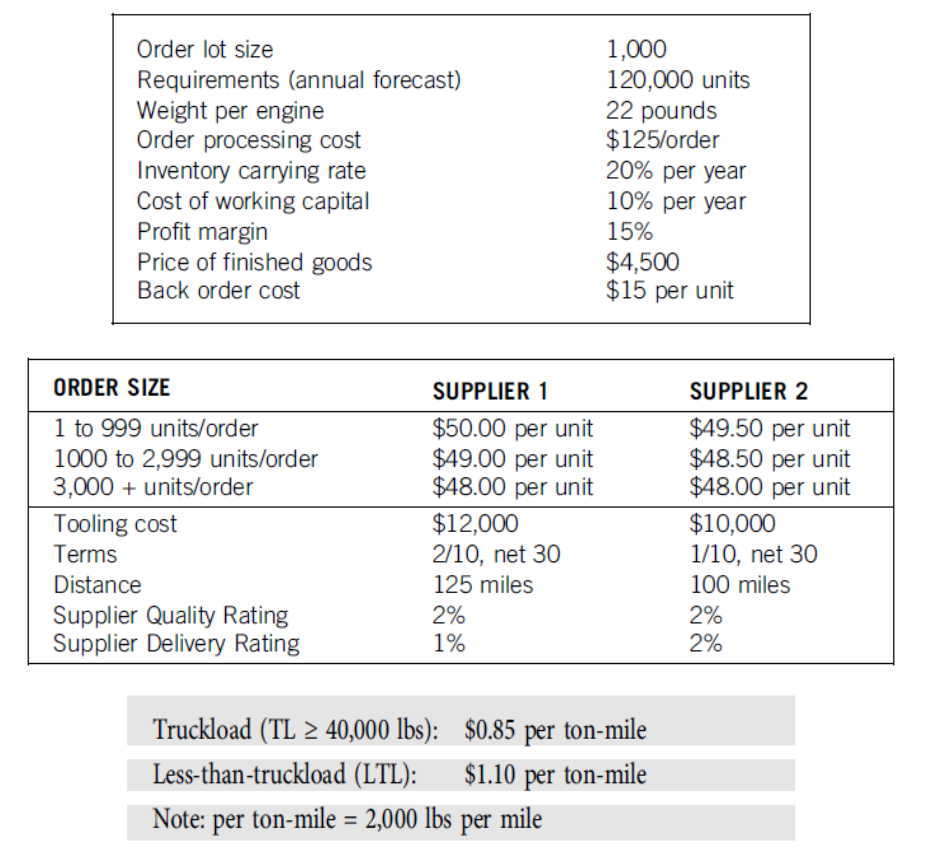
\includegraphics[width=0.75\textwidth]{img2.png}
    \end{figure}
    \begin{solution}
        Based on the provided information, we can construct the following table for ordering and managing the total costs:

        % \begin{center}
        %     \begin{longtable}{| p{2.5cm} | p{4.5cm} | p{4.5cm} |}
        %         \hline
        %         \rowcolor{light-gray} \textbf{Description} & \textbf{Supplier 1} & \textbf{Supplier 2} \\ \hline
        %         \hline
        %         \raggedright Total Engine Cost & 120000 * 49 = 5,880,000 & 120000 * 48.5 = 5,820,000 \\ \hline 
        %         Cash Discount & & \\ \cline{2-3}
        %             \hspace*{10mm}n/30 & 5,880,000 * 10\% * 30/360 = 49,000 & 5,820,000 * 10\% * 30/360 = 48,500 \\ \cline{2-3}
        %             \hspace*{10mm}n/20 & 5,880,000 (10\% * 10/360 + 2\%) = 133,933.33 & NA \\ \cline{2-3}
        %             \hspace*{10mm}n/10 & NA & 5,820,000 (10\% * 10/360 + 1\%) = 74,366.67 \\ \cline{2-3}
        %         \raggedright Largest Discount & 133,933.33 & 74,366.67 \\ \hline
        %         Tooling Cost & 12,000 & 10,000 \\ \hline 
        %         Transportation Cost & 125 miles * 120,000 units * 22lb * 1.1/2000 = 181,500 & 100 miles * 120,000 units * 22lb * 1.1/2000 = 145,200 \\ \hline
        %         Ordering Costs & (120,000 units)/(1000 units/order) * 125 order cost = 15,000 & (120,000 units)/(1000 units/order) * 125 order cost = 15,000 \\ \hline
        %         Carrying Costs & (1000/2) * 49 * 20\% = 4900 & (1000/2) * 48.5 * 20\% = 4850 \\ \hline
        %         Quality Costs & 5,880,000 * 2\% quality rating = 117,600  & 5,820,000 * 2\% quality rating = 116,400 \\ \hline
        %         Delivery Rating & & \\ \cline{2-3}
        %             Backorder (40\%) & 120,000 units * 1\% delivery rating * 40\% backorder * 15 backorder cost = 7,200 & 120,000 units * 2\% delivery rating * 40\% backorder * 15 backorder cost = 14,400 \\ \cline{2-3}
        %             \raggedright Lost Sales (60\%) & 120,000 * 1\% * 60\% * 4500 price finished * 15\% profit margin = 486,000 & 120,000 * 2\% * 60\% * 4500 price finished * 15\% profit margin = 972,000  \\ \hline
        %             & & \\ \hline
        %             \rowcolor{light-gray} \textbf{Total Cost} & 6,570,266.67 & 7023483.33 \\ \hline
        %     \end{longtable}
        % \end{center}
        \begin{center}
            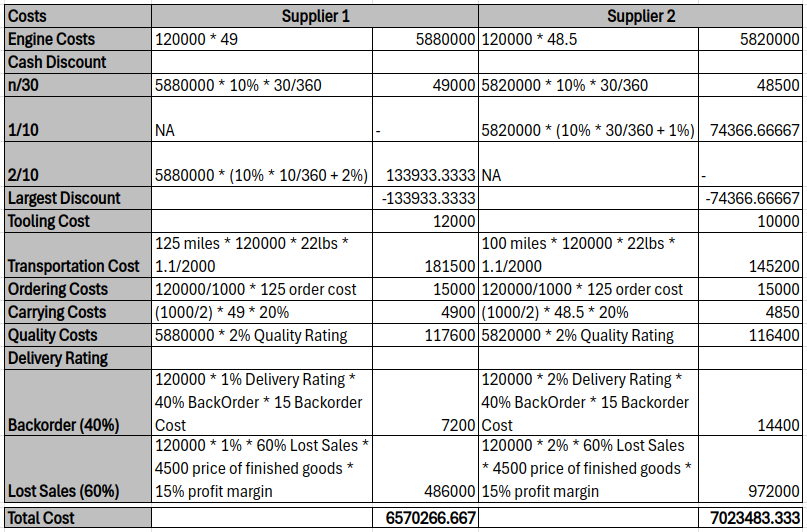
\includegraphics[width=\textwidth]{tca_1.png}
        \end{center}
        Via Total Cost Analysis, we can clearly see that Supplier 1 is more cost-effective as the total cost of ownership is \$6,570,266.67 compared to \$7,023,483.33 for Supplier 2.
    \end{solution}

    \pagebreak
    \question A buyer received bids and other relevant information from three suppliers for a vital component part for its latest product. Given the following information, use total cost analysis to determine which supplier should be chosen. Late delivery of the component results in 70 percent lost sales and 30 percent back orders of finished goods.
    \begin{figure}[ht]
        \centering
        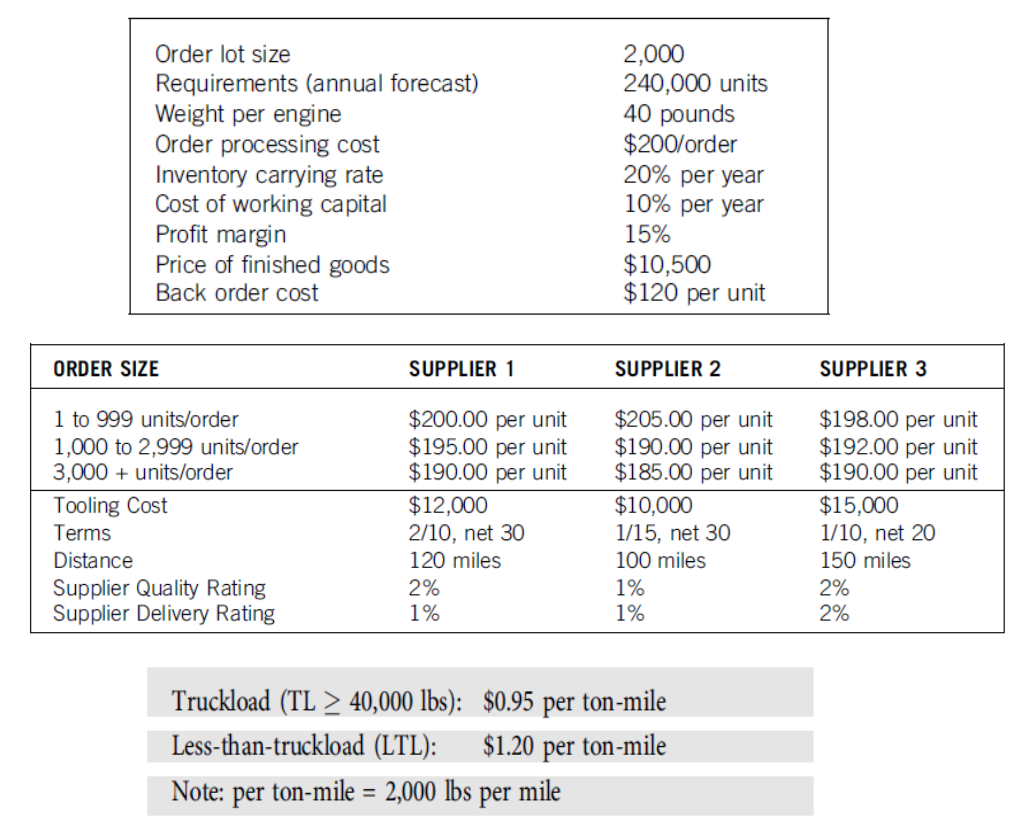
\includegraphics[width=0.75\textwidth]{img3.png}
    \end{figure}
    \begin{solution}
        We use the same methodology as in the previous question to construct a table for the three suppliers as follows:
        % \begin{center}
        %     \begin{longtable}{|p{2cm}|p{3.25cm}|p{3.25cm}|p{3.25cm}|}
        %         \hline 
        %         \rowcolor{light-gray} \textbf{Description} & \textbf{Supplier 1} & \textbf{Supplier 2} & \textbf{Supplier 3} \\ \hline
        %         Total Engine Cost &\raggedright 240,000*195 = 46,800,000 &\raggedright 240,000*190 = 45,600,000 & 240,000*192 = 46,080,000 \\ \hline
        %         \raggedright Cash Discount &  &  & \\ \cline{2-4}
        %         \hspace*{10mm} n/30 &\raggedright 46,800,000 * 10\% * 30/360 = 390,000 &\raggedright 45,600,000 * 10\% * 30/360 = 380,000 & 46,080,000 * 10\% * 20/360 = 256,000 \\ \cline{2-4}
        %         % \hspace*{10mm} n/20 & 1,066,000 & NA & NA \\ \cline{2-4}
        %         % \hspace*{10mm} n/15 & NA & \raggedright 45,600,000 (10\%*15/360+1\%) = 646,000 & NA \\ \cline{2-4}
        %         % \hspace*{10mm} n/10 & NA & NA & 588,800 \\ \cline{2-4}
        %         \raggedright Largest Discount & 1,066,000 & \raggedright 45,600,000 (10\%*15/360+1\%) = 646,000 & 588,800 \\ \hline
                
        %         Tooling Cost & 12,000 & 10,000 & 15,000 \\ \hline

        %         Transportation Cost & \raggedright 120 * 240,000 * 40 * 0.95/2000 = 547,200 &\raggedright 100 * 240,000 * 40 * 0.95/20000 = 456,000 & 150 * 240,000 * 40 * 0.95/2000 = 684,000 \\ \hline

        %         Ordering Costs &\raggedright (240,000)/(2000) * 200 = 24,000 &\raggedright (240,000)/(2000) * 200 = 24,000 & (240,000)/(2000) * 200 = 24,000 \\ \hline

        %         Carrying Costs & (2000/2) * 195 * 20\% = 39,000 & (2000/2) * 190 * 20\% = 38,000 & (2000/2) * 192 * 20\% = 38,400 \\ \hline

        %         Quality Costs & 46,800,000 * 2\% = 936,000 & 45,600,000 * 1\% = 456,000 & 46,080,000 * 2\% = 921,600 \\ \hline

        %         \raggedright Delivery Rating &  &  & \\ \cline{2-4}
        %         \raggedright Backorder (30\%) & 240,000 * 1\% * 30\% * 120 = 86,400 & 240,000 * 1\% * 30\% * 120 = 86,400 & 240,000 * 2\% * 30\% * 120 = 172,800 \\ \cline{2-4}
        %         \raggedright Lost Sales (70\%) & 240,000 * 1\% * 70\% * 10,500 * 15\% = 2,646,000 & 240,000 * 1\% * 70\% * 10,500 * 15\% = 2,646,000 & 240,000 * 2\% * 70\% * 10,500 * 15\% = 5,292,000 \\ \hline

        %         \rowcolor{light-gray} Total Cost & 50,024,600 & 48,670,400 & 52,639,000\\ \hline
        %     \end{longtable}
        % \end{center}
        \begin{center}
            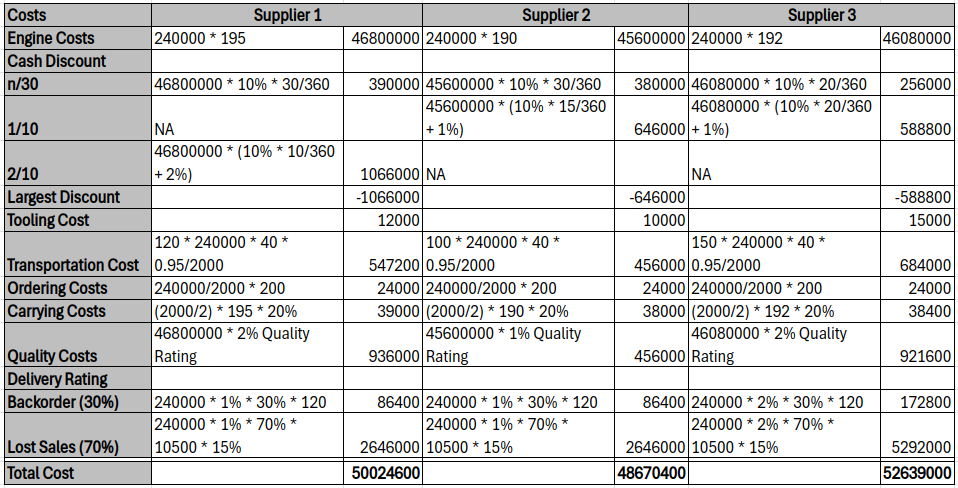
\includegraphics[width=\textwidth]{tca_2.png}
        \end{center}

        From the table above, we can see that Supplier 2 is the most cost-effective option with a total cost of \$48,670,400 compared to \$50,024,600 for Supplier 1 and \$52,639,000 for Supplier 3.

    \end{solution}
\end{questions}

\end{sloppypar}
\end{document}

